\documentclass[11pt,preprint]{aastex}
 %\documentclass[12pt]{emulateapj}
\usepackage[margin= 1.0in]{geometry}    % See geometry.pdf to learn the layout options. There are lots.
\geometry{letterpaper} % or letter or a5paper or ... etc
\usepackage{float}
\usepackage{amssymb,amsmath}
\usepackage[]{epsfig,graphicx}
\usepackage{color}
\usepackage{verbatim}
\DeclareGraphicsRule{.tif}{png}{.jpg}{`convert Num1 `dirname Num1`/`basename Num1 .tif`.jpg}
\newcommand{\units}[1]{\ensuremath{\, \mathrm{#1}}}
\usepackage{enumitem}
\usepackage{natbib}
\newcommand{\degree}{\ensuremath{^\circ}}
\usepackage[maxfloats=25]{morefloats}
\usepackage[normalem]{ulem}
\usepackage{hyperref}
\usepackage{ amssymb }
\newcommand{\TRANSPOSE}{\ensuremath{T}}

\bibliographystyle{apalike}


\begin{document}
\title{Music Recommendation System Using the Million Song Dataset}

 \author{Jordan Rosenblum, Justin Law, \& Erin Grand}
 \affil{Data Science Institute, Columbia University, New York, NY 10027}
 
\date{\today}             

\begin{abstract}
We attempted to build a recommendation system to recommend songs to users using data from the Million Song Dataset available on Kaggle. The main focus of this paper was to use collaborative filtering algorithms that only utilize user feedback in order to predict what songs users may like. For benchmarking the algorithms, we used the same Mean Average Precision score truncated at 500 recommended songs that was used in the original Kaggle competition. It was discovered that probabilistic matrix factorization with a MAP value of 0.014 did not improve results much from using a baseline of simply recommending popular songs, while artist-based popularity along with user-based and item-based collaborative filtering methods yielded much better results with the best method giving a MAP value of 0.048.

%We attempt to build a recommendation system for a subset of the Million Song Dataset. We explore various algorithms including matrix factorization, user-based collaborative filtering, and item-based collaborative filtering. In each case we recommend the top 500 songs that our algorithm returns to each user and compare against the testing set of what the user actually listened to. Matrix factorization gives the worst results, only slightly above the popularity baseline, while artist-based popularity and user-based and item-based collaborative filtering methods yield better results.
\end{abstract}

\tableofcontents

\section{Introduction}
With an increasing amount of accessible data, recommendation systems are becoming more viable and important in various industries including retail, entertainment, and even dating. Recommendation systems allow for services to extend their reach to customers by allowing their users to discover things of interest. Hence, there is a strong interest in implementing a good recommendation system so that their user base can grow. It can be said that building such a system is even more important for the music industry because the entire library of artists and songs are far larger as compared to something like the movie industry so recommending the right music to a specific user is an even harder task. On the other hand, with the shift from a traditional distribution model utilizing physical CDs or records to digital models where users stream or acquire music from internet services, it is now easier than ever to track user preferences and this presents a new opportunity to better predict and recommend songs to users.

In building a recommendation system, various trade-offs had to be accounted for in the type of models that need to be fit. For example, some methods focus more on the metadata of the users and songs (i.e. content-based) such as user or song characteristics (e.g. age, genre, location, etc.) while other methods use a collaborative filtering approach where a user feedback system such as a star rating is used without considering other metadata. In this paper, the latter approach is the focus.

While songs are typically grouped into genres, it is harder to quantify exactly how similar a song is to another and what characteristics of songs a user actually prefers. Two songs by the same artist can produce very different feedback from the same user and thus, determining the exact similarity between two songs is no easy task. The benefit of collaborative filtering methods is that we assume that the tastes of a user can be estimated to be similar to another user and thus we can recommend the songs that the second user has enjoyed to the first user.

\subsection{Data and Statistics}
The main data source for this project is the Million Song Data Set (MSD)  \citep{Bertin-Mahieux2011}. We used the sample data set from the Kaggle competition which contains tuples of user id, song id, and play count. We also used data which links songs to artists through track ids to calculate the artist-based popularity baseline MAP score. The links to all these datasets can be found in the Appendix.

The sample data set had $110000$ users, $163206$ songs, and the number of play counts for each user and song pair. The statistics are summarized in Table \ref{tab:stats}:

\begin{table}[h]
\begin{center}
\begin{tabular}{lll}
\hline
Measurement & \# of Listeners Per Song & \# of Songs Played Per User \\
\hline
Mean  &     8.890194 & 13.190300  \\
Std      &    46.780258 & 8.070827 \\
Min      &    1.0  & 5.0  \\
Max     &   5043 &  53 \\
\end{tabular}
\caption{Basic summary statistics for the full data set.}\label{tab:stats}
\end{center}
\end{table}

The scale of the data was too large to explore on our computers for the algorithms that we used, so we subset the data down to a size easily handled by an average laptop. 
It can be seen in Figure \ref{fig:csongs} that the majority of the songs were listened to by very few users so we were able to decrease the number of songs in our subset without losing all of the play counts. 

\begin{figure}[H] %  figure placement: here, top, bottom, or page
   \centering
   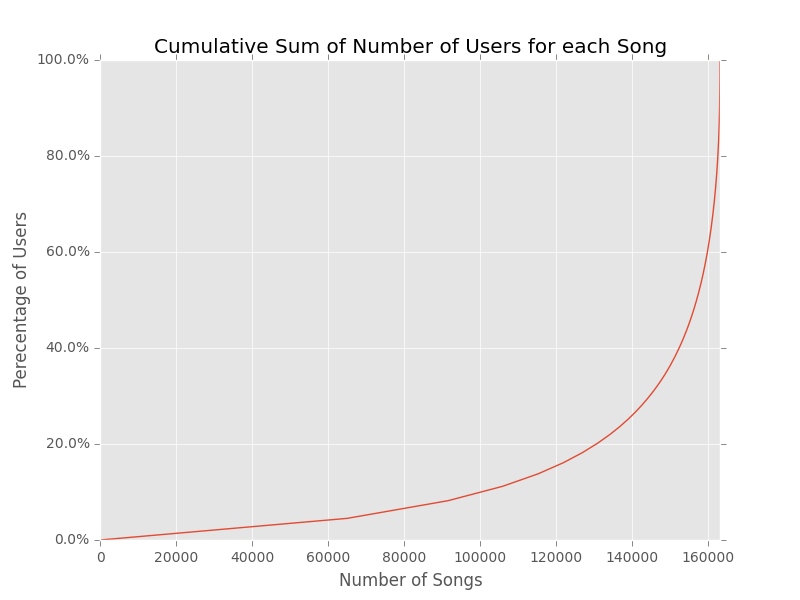
\includegraphics[width=4in]{../plots/final/cumsum-songs.png} 
   \caption{Percentage of users accounted for versus songs with increasing number of plays.}\label{fig:csongs}
\end{figure}

We chose to subset the data to users who have listened to more than 27 songs and songs which were listened to by more than 22 users. This resulted in a dataset which was 10\% the size of the original. The sparsity of the data was .0016, meaning that we only had play counts for 0.16\% of the user-song pairs (i.e. not all users listen to all songs). Despite subsetting the data, though, we are still dealing with $8130$ users and $11861$ songs, so some of our algorithms will take a fair amount of time to run.

%\begin{figure}[htbp] %  figure placement: here, top, bottom, or page
%   \centering
%   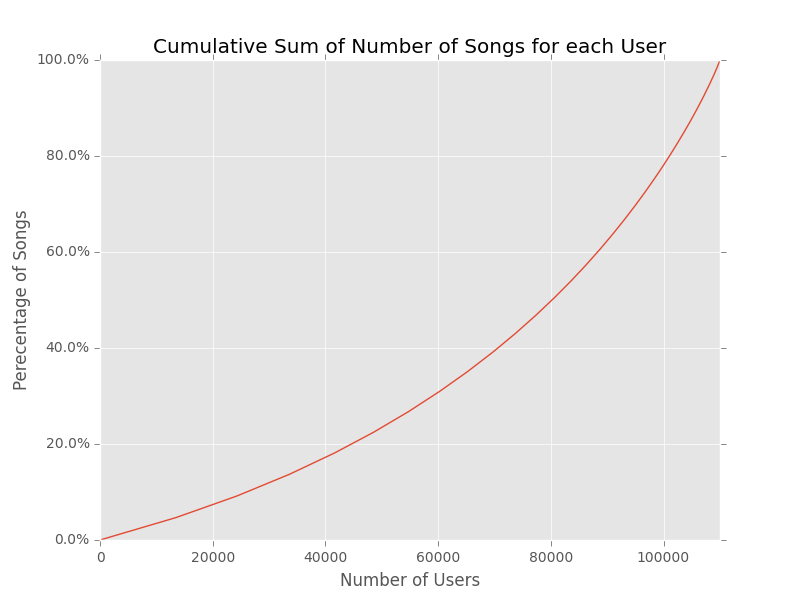
\includegraphics[width=4in]{../plots/final/cumsum-users.png} 
%   \caption{Percentage of songs accounted for versus users with increasing number of plays.}
%   \label{fig:t}
%\end{figure}

%\begin{figure}[htbp] %  figure placement: here, top, bottom, or page
%   \centering
%   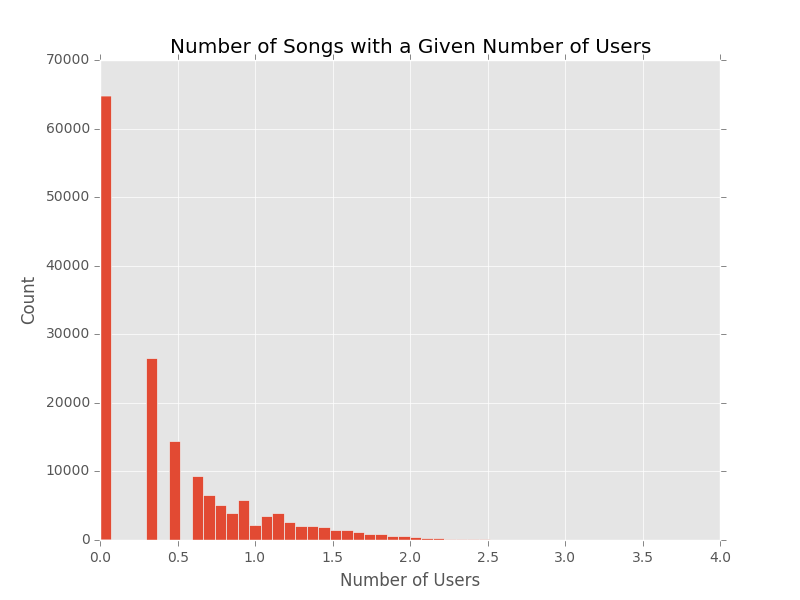
\includegraphics[width=4in]{../plots/final/hist-song.png} 
%   \caption{ }
%   \label{fig:t}
%\end{figure}
%
%\begin{figure}[htbp] %  figure placement: here, top, bottom, or page
%   \centering
%   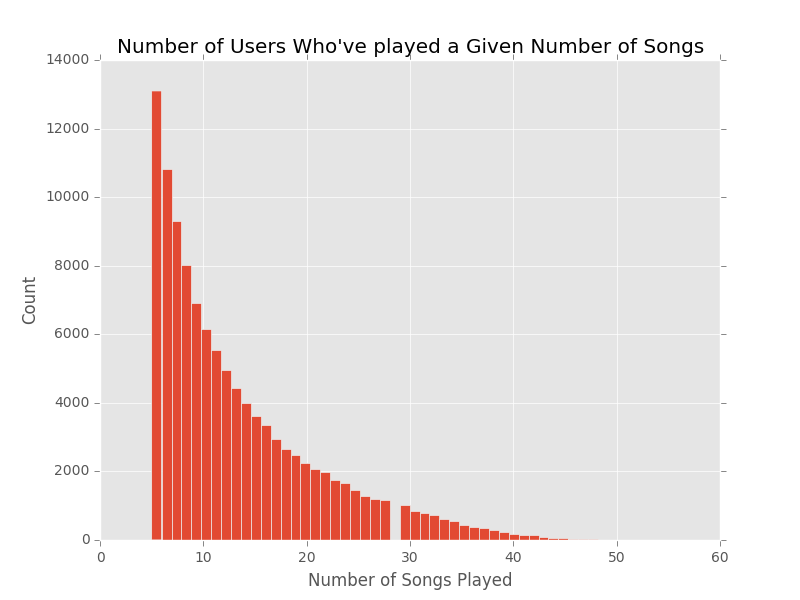
\includegraphics[width=4in]{../plots/final/hist_user_song_count.png} 
%   \caption{ }
%   \label{fig:t}
%\end{figure}


\subsection{Data Analysis}
In order to perform the analysis, we had to fill in training and testing matrices which contained play counts for user and song pairs. We did a random sampling of 80\%/20\% to produce training and testing sets. Next, we implemented various algorithms on the dataset in order to recommend songs to users, including matrix factorization, user-based collaborative filtering, and item-based collaborative filtering.

\subsection{Testing}
We benchmarked our algorithms using a mean average precision score truncated at 500 (MAP@500) for each algorithm. This choice of benchmark was mainly due to MAP@500 also being used as the main method to evaluate algorithms submitted for the Kaggle MSD challenge \citep{McFee:2012:MSD:2187980.2188222}.

Specifically, MAP@500 scores take into account the first 500 recommendations given to each user. Generally, the score looks at the precision for a list of 500 song recommendations for a user and calculates the amount of correct recommendations (true positives) against the total amount of recommended songs. This was done by calculating the average precision at each element in the list of recommended items (i.e. percentage of correct items among first $k$ recommendations) and averaging these for the first 500 recommendations (i.e. for each $k \in \{1, ..., 500\}$, calculate the precision and average them together). Then, the average score is simply calculated by taking the average score over all users.

Intuitively, the score looks at the percentage of recommendations that were in-line with what the user actually liked using the testing set that were not used by the algorithms during training. This score also takes into account the order of the songs recommended so it is desirable to have the song with the highest confidence to be liked at the beginning of the recommendation list. For example, if a user had a test set list of five songs, recommending these five songs at the very beginning would give a MAP score of 1 while recommending them at the very end of the 500 songs would only produce a MAP score of 0.0060. The MAP score can be said to be similar to the AUC of the ROC curve discussed in class without taking into account the order of recommendations.

Two different baseline benchmarks based on \citet{McFee:2012:MSD:2187980.2188222} were used. The first was to simply recommend the top 500 most popular songs in the training dataset to every user with no user personalization. This naive method produced a MAP score of 0.0138 if the top 500 songs were based on the numbers of users who listened to the song or 0.0126 if the top 500 songs were based on the number of total plays the song had. The second baseline used had the bare amount of user personalization where the most popular songs from the artists that the user had also listened to were ordered first. Although this method was also relatively simple and naive, it resulted in a very significant improvement of the MAP score to produce a value of 0.0448.

\section{Algorithms}

\subsection{Probabilistic Matrix Factorization}
Probabilistic matrix factorization (PMF) is a type of collaborative filtering algorithm that can be used to build a recommendation system for users based on user feedback of objects (in this case songs). This allows us to recommend songs to users based on their listening history without the need for content based approaches. 
Training and testing matrices were constructed, of which both have $N_1$ users (rows denoted by $u_i$) and $N_2$ songs (columns denoted by $v_j$). As users have only listened to a fraction of all the songs available, the matrices are sparse, containing zeros in all entries except for those in which a user (representing a single row) has listened to. The goal of matrix factorization is to factor the training matrix into the product of two matrices $U$ and $V$.  The matrix $U$ is $N_1 \times d$ and the matrix $V$ is $d \times N_2$. Another goal of matrix factorization is typically to learn a low-rank factorization of the original matrix while restricting the patterns that are generated in the product of the factorized matrices (e.g. if a user likes a song in a specific group of songs, the user may also like other songs in that group of songs). The choice of $d$ can be subjective but $20$ is a common value to start with. In the factorized matrices, the predicted rating will be $\hat{M}_{ij} = u_i^\TRANSPOSE  v_j$
Using a coordinate ascent algorithm over 100 iterations, each row ($u_i$) and column ($v_j$) of the training matrix is then updated (equations \ref{eq1} and \ref{eq2}) in order to maximize the log joint likelihood (equation \ref{eq3}).

\begin{equation}
u_i = \left( \lambda\sigma^2 I + \sum_{j \in \Omega_{u_i}} v_j v_j^\TRANSPOSE \right)^{-1}\left(\sum_{j \in \Omega_{u_i}} M_{ij} v_{j} \right)
\label{eq1}
\end{equation}

\begin{equation}
v_j = \left( \lambda\sigma^2 I + \sum_{i \in \Omega_{v_j}} u_i u_i^\TRANSPOSE  \right)^{-1}\left(\sum_{i \in \Omega_{v_j}} M_{ij} u_{i} \right)
\label{eq2}
\end{equation}

\begin{equation}
\mathcal{L} = - \sum_{(i,j) \in \Omega} \frac{1}{2\sigma^2} {|| M_{ij} - u_i^\TRANSPOSE  v_j||}^2 - \sum_{i=1}^{N_1} \frac{\lambda}{2} ||u_i^2 || - \sum_{j=1}^{N_2} \frac{\lambda}{2} ||v_j^2 || + \text{constant}
\label{eq3} 
\end{equation}

\emph{Note: $\lambda = 10$ was used and $\Omega$ is the set of all indices in the matrix which have an observation.}

There are several hyperparameters that can be tweaked in order to achieve a better MAP result using matrix factorization. The main ones that we explored were the variance, the rank $d$ of the factorization, and the number of iterations. As the project was being done using Python and the main computational package (\emph{scikit-learn}) did not have probabilistic matrix factorization functions, we decided to apply the algorithm that we wrote ourselves for a different class \citep{koren2009matrix}. It should be noted that while PMF algorithms can be parallelized to significantly improve running time and scaled to handle large amounts of data, being limited to a single machine to run these computations meant that subsetting the data was necessary in order to actually execute the algorithm successfully while limiting computational time to durations that were feasible for exploration.
 
After testing various values of the parameters, it was soon discovered that matrix factorization results were significantly below the popularity baseline and changing the hyperparameters around did not help much. The best MAP value of 0.0039 was achieved using a high rank $d$ of 80 over 100 iterations with a variance of 1.0. The log joint likelihood chart can be used to verify that the probabilistic matrix factorization algorithm is running properly in that the values are monotonically increasing, which corresponds to a decreasing training error. 

The first graph in Figure \ref{defaultPMF} shows that the log joint likelihood is indeed monotonically increasing and slowed down significantly after the first twenty iterations. The second graph in the same figure shows the MAP values from the same run and it shows that the MAP values decreasing after the maximum at five iterations. It could be argued that emphasis should be placed on finding the right number of iterations to produce the best MAP values, but since the overall MAP results were poor and the differences were minimal, it was decided that this was not to be a priority for further experimentation. Due to this conclusion, further exploration of the probabilistic matrix factorization algorithm was limited to 30 iterations in order to reduce computational time.

\begin{figure}[H] %  figure placement: here, top, bottom, or page
   \centering
   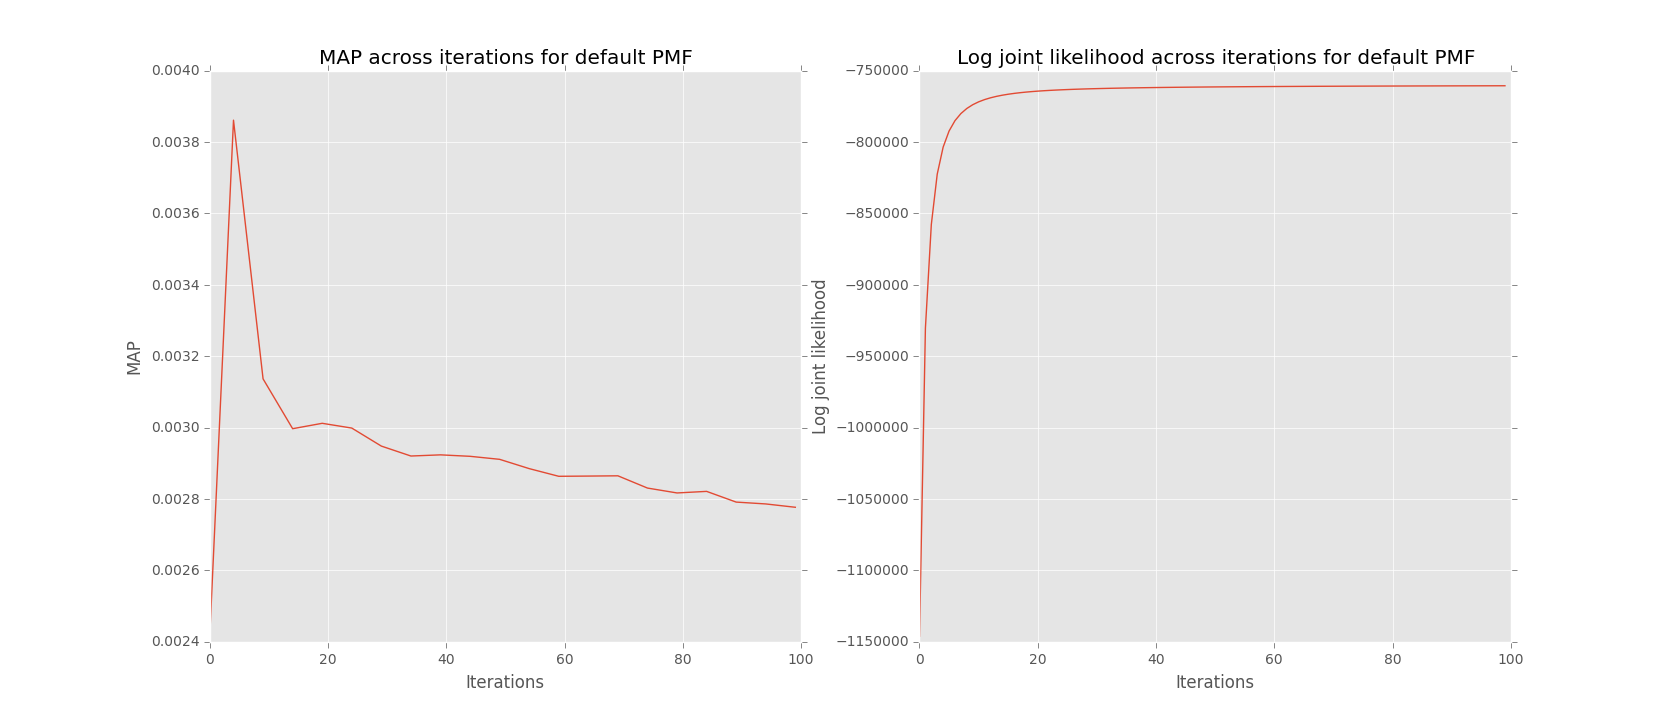
\includegraphics[width=6in]{../plots/final/defaultPMF.png} 
   \caption{MAP values and log joint likelihood values for PMF using default play-count values with $\sigma^2 = 1.0$ and $d = 80$}
   \label{defaultPMF}
\end{figure}
 
One explanation for the very low MAP scores using PMF was that the number of plays that were used were different from the typical bounded ratings PMF is typically used on. Using implicit user feedback (number of plays) instead of explicit user feedback (ratings) has been shown in literature, such as \citet{hu2008collaborative}, to create various issues. One of the main issues is that implicit feedback is inherently noisy and does not measure negative feedback. Listeners may have played a song and simply found out that they disliked the song. The other main issue is that the exact number of plays could have a significantly different meaning across different users. For example, an avid listener who has played a song five times could have a different meaning as compared to a listener that has played songs at most five times.
 
In order to tackle the issue of using implicit user feedback, we tried four different scaling schemas independently. These included normalizing user play counts by the total number of plays for the user, normalizing song play counts by the total number of plays for the song, making the data binary (changing all non-zero play counts to 1), and applying tf-idf. While testing out these schemas, we continued to vary the hyperparameters (i.e. $d$ and variance) in order to determine if they changed the MAP results significantly. 
 
The results from the experiments are shown in Figure \ref{fig:PMF}. It was found that the rank, $d$, did not contribute significantly to the MAP values especially in settings where the MAP values were close to the popularity baseline. Higher variance values were found to significantly increase the MAP values. It can be argued that the reason why the default PMF works best at variance of 10 instead of 1.0 for the others is that the empirical variance of play count values is at least an order of magnitude higher than the others. This also suggests that the variance used in PMF should scale with the empirical variance, but the exact relationship remains unclear.

%\newpage
\begin{figure}[htbp] %  figure placement: here, top, bottom, or page
   \centering
   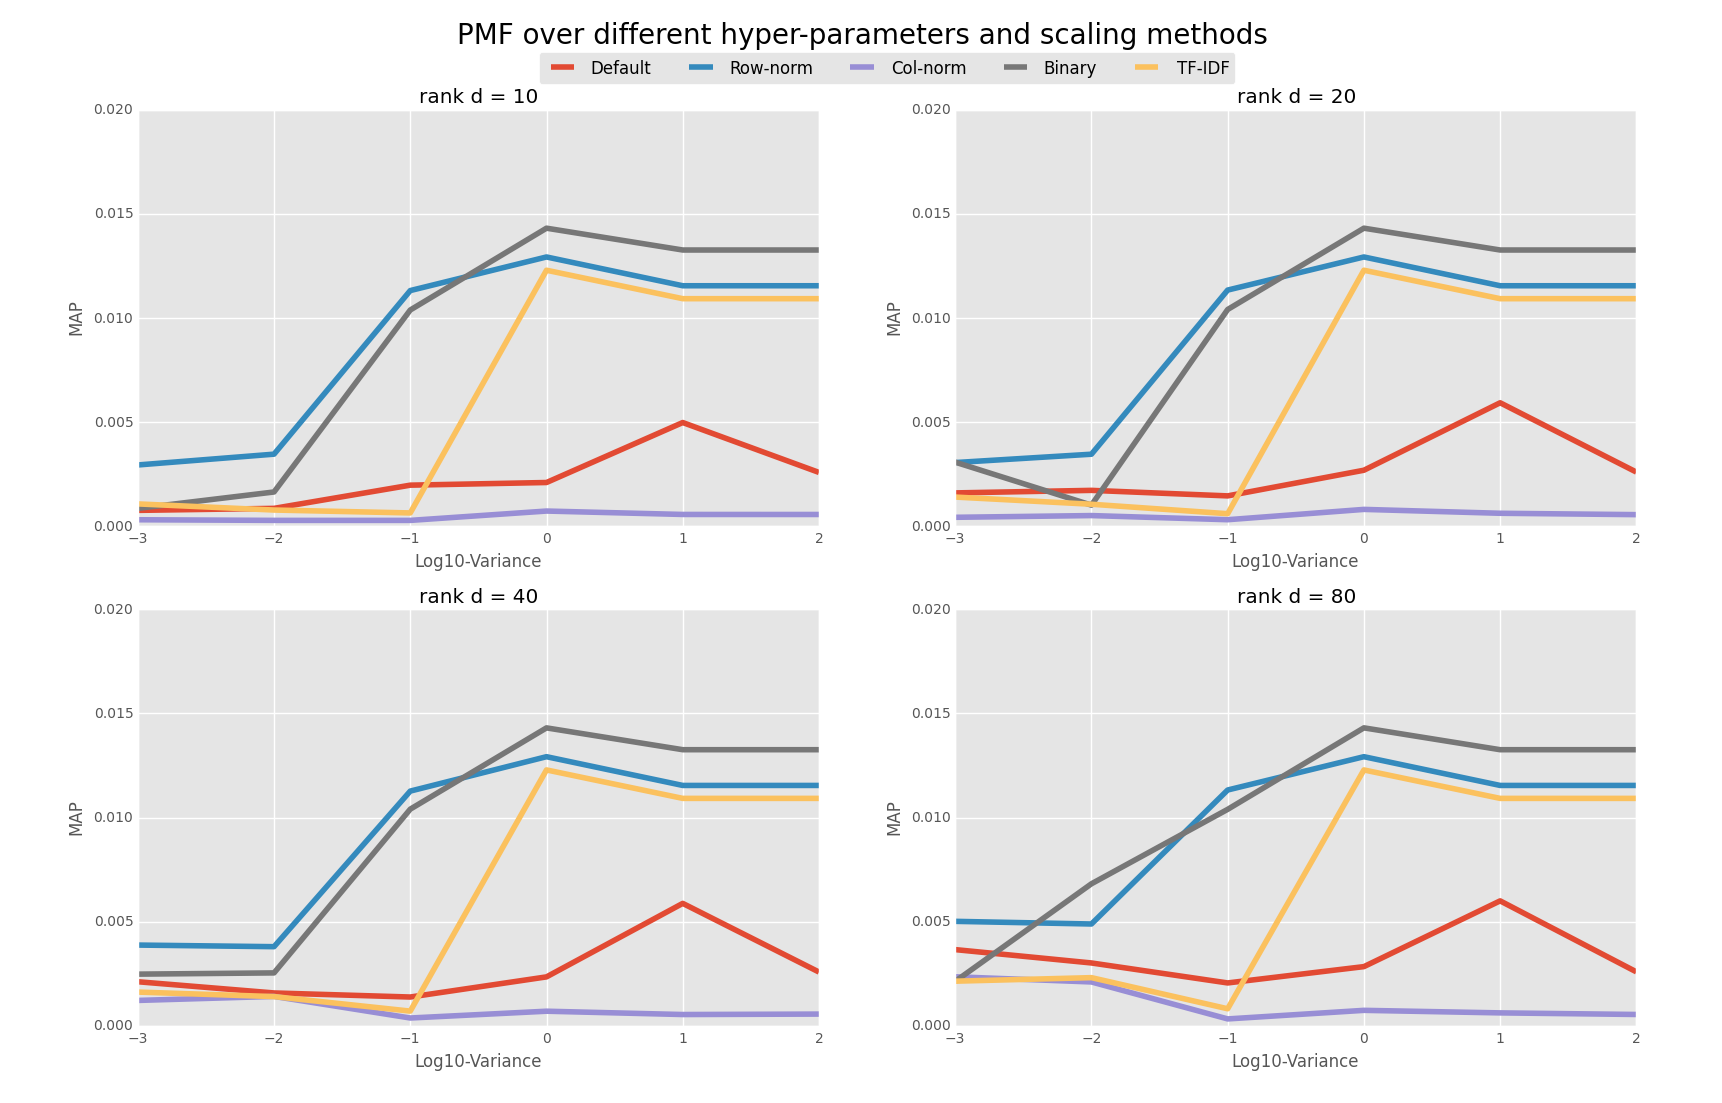
\includegraphics[width=6in]{../plots/final/PMF.png} 
   \caption{MAP values for different scaling methods and hyperparameters after 30 iterations}
   \label{fig:PMF}
\end{figure}

In terms of scaling schemas, making the data binary produced the best result, with the second best being normalizing the data against the total number of plays for each user. Perhaps it can be said that using number of plays introduces more noise than simply considering if the user has played the song or not. Tf-idf performed slightly worse than the two, so down-weighting the songs shared more often by users did not produce better recommendations. Interestingly enough, normalizing the data against total number of plays for each song performed the worst and this most likely relates to the fact that number of plays is more meaningful relative to each user rather than to each song. 
 
Regardless, the best result achieved for PMF in the end was 0.0143, which was only slightly above the popularity baseline. Based on literature review \citep{li2012million, McFee:2012:MSD:2187980.2188222}, we have found that this is better or in line with what others have achieved with using PMF on play counts. Nevertheless, this indicates that PMF is not suitable for the MSD dataset and this can be attributed to the implicit feedback issue or simply to the fact that the dataset is too sparse. A dataset that is too sparse prevents PMF from learning enough information about how users rank songs to produce more accurate recommendations. However, it is still possible to apply matrix factorization techniques to this dataset through using metadata and this has been demonstrated to be viable by \citet{liangcodebook} which achieved MAP values exceeding 0.1.  



\subsection{User Based and Item Based Collaborative Filtering}
%\subsubsection{Intro to Memory-Based Collaborative Filtering}
A simpler set of methods for determining which songs to recommend to individual users is by using user- or item/song- based similarity (both also considered collaborative filtering). These only consider whether or not a user listened to a song and does not take into account the play count. Similarity scores between users (i.e. user-based) and songs (i.e. item-based) were calculated using cosine similarity \citep{aiolli2013preliminary, li2012million}. Intuitively, they work by recommending users songs that other similar users like (user-based) or by recommending songs which are similar to the songs the user has already listened to (item-based). The downside to this method is the computational complexity. Given the quadratic runtime of these algorithms, they are more difficult to scale to a larger dataset. As for storage requirements, we will have to store all pairs of similarity scores for users in the case of user-based and songs in the case of item-based. The details are described below.

\subsubsection{User-Based Collaborative Filtering}
For user-based recommendation, we first calculated the similarity score between every pair of users, $u$ and $v$, using equation \ref{eq:item}:

\begin{equation}
sim(u,v) = \frac{\text{\# common items}(u, v)}{{\text{\# items}(u)}^{1/2} \times {\text{\# items}(v)}^{1/2}}
\label{eq:item}
\end{equation}

Then, for each user, we looked at each song in the dataset and found all other users who have listened to that song. Next, we added up the similarity score of each of those users, $v$, with the original user, $u$, and got the weight for a particular song, $i$:  

$$w_i = \sum_{v \in V} sim(u, v)$$

The sum is a proxy for how likely the user is to like that particular song. This was repeated for all songs and recommended the user the top 500 songs which had the highest scores. This method led to a MAP value of 0.0377.

\subsubsection{Item-Based Collaborative Filtering}
For item-based recommendation, which turned out to be our best algorithm in terms of a MAP value, we first calculated the similarity score between every pair of songs, $i$ and $j$, using equation \ref{eq:user} and saved the most similar songs to each song in the process:

\begin{equation}
sim(i,j) = \frac{\text{\# common users}(i, j)}{{\text{\# items}(i)}^{1/2} \times {\text{\# items}(j)}^{1/2}}
\label{eq:user}
\end{equation}

Then, for each user, we found all the songs listened to. Next, we calculated the most similar songs to each of those songs listened to by the user. If the same similar songs came up multiple times, we added the weights together. In other words, for each song, $b$, that was found to be similar to one of the songs, $a$, that the user listened to, we calculated the score for that song, $b$:

$$w_b = \sum_{a \in A} sim(a, b)$$

Lastly, we sorted the songs by scores and recommended the user the top 500 songs which had the highest scores. This method led to a MAP value of 0.0479.


\section{Results}
After comparing the various algorithms, we found that item-based collaborative filtering gave us the best result. Our most complicated model, matrix factorization, gave us results barely above the popularity baseline. On the other hand, simply recommending users songs by artists they have already listened to (the artist-based popularity baseline) resulted in a significantly better recommendation system. This is probably because users tend to listen to multiple songs by the same artist. Our song-based collaborative filtering technique produced the best results despite it being more naive as compared to matrix factorization. Our final results for each technique employed are summarized in Table \ref{tab:map}. 

\begin{table}[h]
\begin{center}
\begin{tabular}{lc}
\hline
\bf{Algorithm} &  \bf{MAP score}\\ \hline
Item Based  CF  &  0.0479 \\ 
Artist Based Popularity Baseline  & 0.0448    \\ 
User Based  CF  &  0.0377 \\ 
Binary Matrix Factorization  &   0.0143  \\ 
Top 500 Songs by Count  Baseline &  0.0138  \\ 
Top 500 Songs by Plays  Baseline &  0.0126  \\ 
\end{tabular}
\caption{Final MAP results across various algorithms.}\label{tab:map}
\end{center}
\end{table}

\section{Future Work}
Apart from the algorithms discussed above, we also explored building a recommendation system based on K-Means Clustering (by both user and song) and Non-Negative Matrix Factorization (NMF). In the end, both of these methods yielded worse results as compared to Probabilistic Matrix Factorization so we decided not to explore them further. Next steps include incorporating tags and metadata present in the dataset (e.g. year, genre, and audio metadata). It would also be useful to expand the size of the subset and distribute the workload to multiple machines so that more data could be analyzed.

%To Reference a paper: 

%The Million Song Dataset Challenge: \citep{McFee:2012:MSD:2187980.2188222} \\
%Million Song Dataset Recommendation Project Report: \citep{li2012million} \\
%codebook-based scalable music tagging with poisson matrix factorization: \citep{liangcodebook} \\
%Matrix Factorization Techniques for Recommender Systems: \citep{koren2009matrix} \\
%A Preliminary Study on a Recommender System for the Million Songs Dataset Challenge: \citep{aiolli2013preliminary} \\


\newpage
\bibliography{msdref}

\small{
\section{Appendix}

\begin{itemize}
  \item Link to our github repository: \url{https://github.com/eringrand/musicanalysis}
  \item The MSD Kaggle challenge: \url{https://www.kaggle.com/c/msdchallenge}
  \item The user, song, play count dataset: \url{https://www.kaggle.com/c/msdchallenge/download/kaggle_visible_evaluation_triplets.zip}
  \item Data to link songs to artists through track ids: \url{http://labrosa.ee.columbia.edu/millionsong/sites/default/files/AdditionalFiles/track_metadata.db}
\end{itemize}
}

\end{document} 
